\documentclass[12pt]{article}
\usepackage{sectsty}
\usepackage{graphicx}
\usepackage[utf8]{inputenc}
\usepackage{natbib}
\usepackage[hyphens,spaces,obeyspaces]{url}
\usepackage{hyperref}
\usepackage{blindtext}
\usepackage{enumitem}

\title{\textbf{Graph Theory Research}}
\author{\textbf{Conor Shortt}}
\date{\textbf{March 2020}}

\begin{document}
\maketitle
\begin{figure}[h!]
\centering

\includegraphics[scale=0.7]{Photos/logo.jpg}
\end{figure}
\pagebreak
\newpage

\newpage
\tableofcontents
\newpage

\section{Introduction}
This document contains the research I have done as part of my Graph Theory Project. Our project involves writing a program in Python to execute regular expressions on strings using an algorithm known as Thompson’s construction, named after the well-known computer scientist Ken Thompson.

\begin{figure}[h!]
\centering
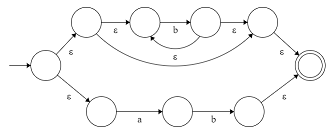
\includegraphics[scale=1]{Photos/nfa.png}
\caption{NFA Example for regex $a.b|b*$}
\label{fig:nfa}
\end{figure}

\subsection{GitHub Repository}
\begin{description}
\item[$\cdot$]{https://github.com/conorshortt123/graphtheory-project-repo}
\end{description}

\newpage
\section{Thompson's Construction}
\begin{figure}[h!]
\centering
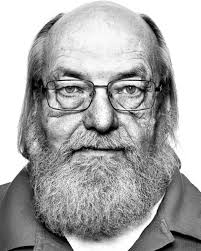
\includegraphics[scale=0.7]{Photos/kenthompson.jpg}
\caption{Ken Thompson}
\label{fig:nfa}
\end{figure}
\cite{wikipedia}
Thompson's construction algorithm, is a way of converting a regular expression into equivalent non-deterministic finite automaton. NFA's are used to match strings against regular expressions. This algorithm is credited to Ken Thompson but can also be called the McNaughton-Yamada-Thompson algorithm.

Regex and NFA's are two representations of formal languages. (A formal language in computer science consists of words whose letters are taken from an alphabet and are well formed according to a specific set of rules.) Text processors use regular expressions to describe advanced search patterns, NFA's are better suited for execution using a computer, therefore Thompson's algorithm has a practical interest in relation to executing regular expressions.
\newpage

\subsection{Example NFA's}
\begin{description}
\begin{figure}[h!]
\centering
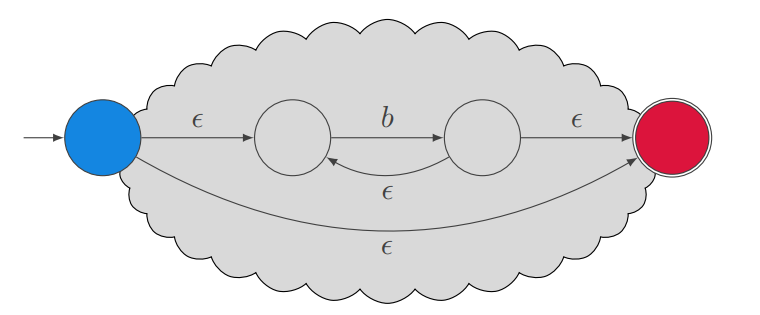
\includegraphics[scale=0.6]{Photos/KleeneStarFrag.png}
\caption{NFA Example for regex $b*$}
\label{fig:nfa}
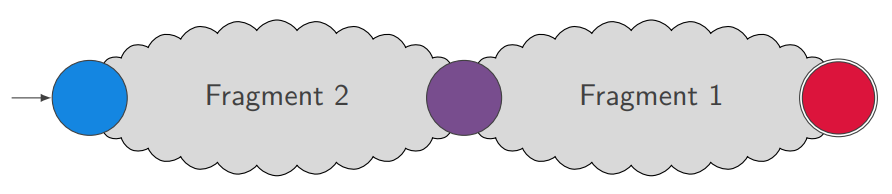
\includegraphics[scale=0.6]{Photos/Concatenation.png}
\caption{NFA Example for a concatenation regex}
\label{fig:nfa}
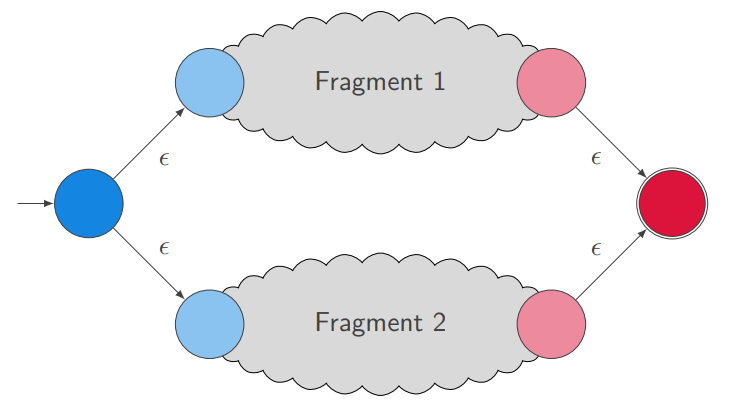
\includegraphics[scale=0.6]{Photos/Union.png}
\caption{NFA Example for a Union regex}
\label{fig:nfa}
\end{figure}
\cite{moodle}
\emph{These are examples of NFA fragments. NFA fragments can be combined together to form larger NFA's.}
\newline\newline
\textbf{Figure 3:}
\newline\newline
As you can see in figure 3, this is an example of an NFA fragment for the Kleene star. The Kleene star is a unary operator, it is widely used for regular expressions, which is the context in which it was introduced by Stephen Kleene to characterize certain automata, where it means "zero or more".
\newline\newline
\textbf{Figure 4:}
\newline\newline
In figure 4 is an example of an NFA fragment for a concatenation regular expression. Concatenation combines fragments so the NFA can use multiple operators.
\newline\newline
\textbf{Figure 5:}
\newline\newline
In figure 5 is an example of an NFA fragment for a union regular expression. The union operator acts as an OR gate, which will accept one of two different inputs.
\newline\newline\newline
There are other operators such as the question mark operator, plus operator, caret operator etc. For the purposes of my particular project I included five operators $( * . | ? +)$. The dot operator in my project is not the standard dot operator used in regular expression engines, it is generally used to match any character bar empty strings, but I used it for concatenation.
\end{description}

\newpage
\section{Common Regular Expression Operators}
\textbf{Match-self Operator}\newline
This operator matches the character itself, for example operator 'A' will match 'A' and only 'A'.
\newline\newline
\textbf{Concatenation Operator}\newline
Concatenates two fragments with each other. Generally, concatenation doesn't have a special operator character, you just put b after a to match the string "ab", but in my python program concatenation is done using the special character '.'
\newline\newline
\textbf{Kleene Star Operator}\newline
This operator repeats the preceding character zero, one, or many times. Therefore this operator will accept an empty string. The regular expression $a*$ will accept strings '', 'a', 'aaaaa' and so on.
\newline\newline
\textbf{Plus Operator}\newline
This operator repeats the preceding character like the Kleene star, but only one or more times, therefore this operator will not accept the empty string.
\newline\newline
\textbf{Question Mark Operator}\newline
This operator matches zero or one of the preceding character. It matches the empty string and also whichever character it is preceding by.
\newline\newline
\textbf{Union Operator}\newline
This operator matches either of the specified fragments. Implemented with the $|$ character. For example, the regex $a*b|c+$ will match either "abbbb" or could also match "cccc".
\cite{MIT}
\newpage

\section{Problem Statement}
\cite{moodle}\cite{ianmcloughlin}\emph{"You must write a program in the Python\cite{python} programming language that can
build a non-deterministic finite automaton (NFA) from a regular expression,
and can use the NFA to check if the regular expression matches any given
string of text. You must write the program from scratch and cannot use the
re package from the Python standard library nor any other external library.
A regular expression is a string containing a series of characters, some of
which may have a special meaning. For example, the three characters ., |,
and * have the special meanings concatenate, or, and Kleene star respectively.
For example, the regular expression 0.1 means a 0 followed by a 1, 0|1 means
a 0 or a 1, and 1* means any number of 1’s. These special characters must
be used in your submission.
Other special characters you might consider allowing as input are brackets
() which can be used for grouping, + which means at least one of, and ? which
means zero or one of. You might also decide to remove the concatenation
character, so that 1.0 becomes 10, with the concatenation implicit. You may
initially restrict the non-special characters your program works with to 0 and
1. However, you should at least attempt to expand these to all the digits,
and the characters a to z, and A to Z."}

\subsection{Steps to Solve Problem Statement}
\begin{itemize}[noitemsep]
\item Take in two \textbf{inputs}, the \textbf{regular expression} and the \textbf{string} the user wishes to match against the regex
\item Use the \textbf{shunting yard algorithm} to convert the regular expression from \textbf{infix} to \textbf{postfix}
\item Create \textbf{NFA fragments} by popping characters off the postfix stack until you are left with a \textbf{singular NFA}.
\item Read in the user \textbf{input string} into the NFA and \textbf{follow all epsilon arrows}, once user string is finished being read \textbf{return accept states}.
\item If there are \textbf{accept states returned} then the \textbf{regular expression matches the input string.}
\end{itemize}

\section{Conclusion}
There are many ways to approach the problem. In my solution on my Github repository as highlighted in sub section 1.1, you will find implemented a full string match against the regular expression. In general, regular expressions are used to search for partial strings. In future I expect I will expand on my program and further add partial string matching and also add in many more operators that standard regular expression engines have to offer.

\newpage
\bibliographystyle{plain}
\bibliography{references}
\end{document}